% !TeX root = ../main.tex

% Overview
% Explain the system overview
% Design goals
% Explain the system workflow
% Identify system components and explain their function
\chapter{Overview}\label{chapter:overview}
In this chapter, we aim to provide a clear overview of our project, outlining its progression, design goals, and its key components.
We'll begin by discussing the shifts in direction that the project has taken, due to our new insights.
This reflection is quite important as we have come to notice that our first assumption was erroneous.
Next, we will talk a bit bout the design goals when extending the verifer.
Following this, we will give an overview of how the whole verifier/reproducer combination works along with how individual components function.

\section{Course of the Project}
We started this project by evaluating the accuracy and reliability of various emulators.
This entailed research into common emulator bugs along with recreating them.
Our main targets were \ac{QEMU} and Arancini and most of our research was on them.

Our part in this project was focused on developing a program that could produce tests by utilizing symbolic execution on erroneous programs.
Initially, we assumed that a significant proportion of the flaws and inconsistencies discovered in \ac{QEMU} could be attributed to issues within the \ac{TCG}.

Specifically, we suspected that these bugs were a result of erroneous execution paths that led to incorrect jumps within the code. To address this, we planned to use symbolic execution to construct a tree.
This tree was intended to serve as a map, guiding us through the execution path and therefore identifying these incorrect jumps.

Through this method, we had hoped to:
\begin{enumerate}[label=(\Alph*)]
   \item Find the shortest path to the error
   \item Recreate the erroneous program by changing the inputs and making sure that it follows the aforementioned path
\end{enumerate}

Through this method, we had hoped to automate test generation and simplify finding bugs in emulators.
However we came to notice that most of the bugs stemming from \ac{TCG} were not because of incorrect jumps, they were in fact caused by wrong implementation of instructions.
Because of these findings, our project had a slight change of direction.

Because of our new findings, we stopped concentrating on following the erroneous path and instead concentrated on the offending instruction.
Considering that most of the hard-to-find bugs stem not from the general functionality but the edge cases, we came to the understanding that we need to recreate the state where this bug occurs.
This meant we needed to sample the memory and registers before the erroneous instruction.
We used symbolic execution to find the symbolic expressions that were used in the instruction and then used concrete values to recreate a similar state.
By combining these values, the offending instruction, and other code stubs that are used for running code, we managed to recreate a tiny executable that can cause the same bug.

\section{Design Goals}
Our main design goal for the reproducer was to extract bugs in the simplest manner possible.
This meant the reproducer should need only the minimal amount of data and the resulting program should be as simple as possible.
We hoped to replicate the bugs by utilizing only the provided symbolic traces and concrete values.

We also tried to abstract the environment of the bug from the required assembly instructions.
This meant we tried to design the reproducer such that it could produce parts of the environment, for example, stack, registers, or memory layout without necessarily turning it to assembly instructions.
We tried to make this information as flexible as possible to facilitate easier analysis.

\section{System Workflow and Component's Functions}
The reproducer is designed as an add-on to the Focaccia.
Much of its functionality relies on this verifier.
As shown in the figure \ref{fig:ver_and_rep_1} all the inputs for the reproducer come from it.

\begin{figure}[ht]
   \centering
   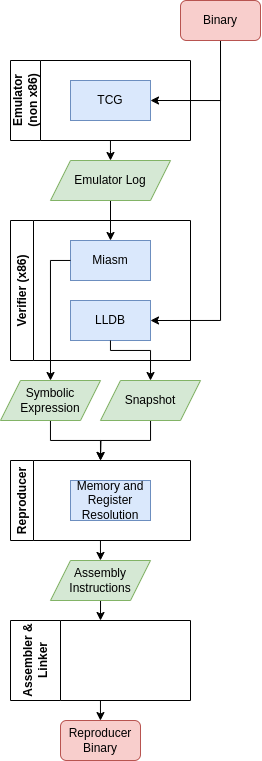
\includegraphics[width=0.45\linewidth]{figures/ver_and_rep_1}
   \caption[Verifier and reproducer]{Overview of the verifier and the reproducer}
   \label{fig:ver_and_rep_1}
\end{figure}

\subsection{Inputs}
Both the verifier and the reproducer depend on the same two inputs, namely the emulator log and the binary.
However, there are some peculiarities for both of them.
The first one is the emulator log, which can be structured in any way, as long as it contains the necessary information.
These logs should either document every change in memory and register values based on the program counter \ac{PC} or provide complete snapshots of memory and register states at each PC.
These are necessary as Focaccia relies on these logs to accurately replicate the emulator's actions.

Also, the logs we use must come from binaries that are statically linked, not dynamically linked.
This ensures that the program runs with the same set of instructions, regardless of the environment it's executed.
For instance, discrepancies in the \ac{clib}, whether due to different libraries or versions, can lead to varied instructions.
Such variations would cause the traces to not align, resulting in a trace output filled with errors unrelated to the actual faulty instruction.

\subsection{First Component: Focaccia the Verifier}

Focaccia is the verifier that we are using to detect errors in the emulators.
It functions by comparing an emulator with an oracle.
It uses the Miasm reverse engineering framework and the LLDB debugger from LLVM. 
There are two inputs required for the verification, namely the emulator log and the binary.
Firstly, Focaccia analyzes the instructions in the binary to generate a symbolic trace.
This trace maps out all modifications in memory, registers, and branches, effectively creating a tree-like structure that outlines potential changes for each instruction.
However, this symbolic trace isn't sufficient on its own. 
The binary also provides concrete values, from which Focaccia takes snapshots.
Later these transformations are compared with the emulator log.
Then it compares the transformations and finds whether there is a mismatch between different states.

\subsection{Second Component: the Reproducer}
The reproducer is an add-on to the verifier, with its role being to prepare the assembly instructions needed for triggering a specific bug. 
If enabled by the verifier, it will be run after the verification process is done and the erroneous instructions are found.
After the verifier finishes collecting the snapshots and the symbolic expressions.
It is filtered for discrepancies and if found it is passed to the reproducer as shown in figure \ref{fig:ver_and_rep_1}.
After the reproducer receives the inputs, it will then try to extract only the necessary data from the snapshot which will be bundled with other assembly instructions.
This output is significant as it not only points out which instruction is erroneous but also demonstrates the conditions under which the bug occurs.
Ultimately it should make debugging easier by recreating both the environment and the instructions.


